\chapter{Dữ liệu} \label{chap-Data}

\section{Thu thập dữ liệu}
Hiện nay đa số  các sàn giao dịch lớn như Binance, Huobipro, OKCoin đều cung cấp api hỗ trợ cho phép xem lại các OrderBook, tỷ giá giao dịch các phiên trước đó, đặt lệnh giao dịch. Như đã đề cập ở chương 1, trong phạm vi sàn nghiên cứu của đề tài, chúng tôi chọn sàn Binance và các đồng cơ bản là BTC, ETH, USDT, BNB để nghiên cứu; Thông qua tìm hiểu, có hai thư viện hỗ trợ thu thập thông qua api trên sàn biannce là python-binance do sàn viết và ccxt (đã được Binance chứng nhận) đều được viết bằng ngôn ngữ python. Ccxt với khả năng hỗ trợ hơn 120 sàn khác nhau, hỗ trợ với nhiều ngôn ngữ lập trình, chính vì vậy ccxt được chọn làm thư viện chính để  thu thập dữ liệu và tạo các lệnh giao dịch để có thể mở rộng đề tài trong tương lai.\\
Để dễ hình dung về chức năng của api, api được ccxt chia thành hai loại là:
\begin{itemize}
    \item Public api: hỗ trợ lấy tickers, OrderBook; tỉ giá cặp tại thời điểm trước; các giao dịch trong khoảng thời gian trước đó.
    \item Private api: hỗ trợ tạo, hủy lệnh giao dịch; lấy các lệnh giao dịch trước đây; xem số đồng trong các ví của tài khoản sở hữu api này.
\end{itemize}
Quá trình chuẩn bị dữ liệu được thực hiện thông qua public api.\\
Khác với sàn giao dịch truyền thống (sàn chứng khoán), sàn giao dịch tiền mã hóa hoạt động liên tục vì vậy việc chia phiên giao dịch được sàn định nghĩa theo các khoảng thời gian cụ thể theo mặc định như 1 phút, 1 giờ, 1 ngày,... Điều này giúp cho người tham gia có thể biết tỷ giá trong các phiên giao dịch trước. Tuy nhiên trong phiên giao dịch có thể gồm nhiều các giao dịch với giá, số lượng đồng khác nhau. Nhằm dễ  thống kê, public api cung cấp để lấy giá OHLCV( Open, High, Low, Close, Volume) tương ứng với giá mở sàn; giá cao nhất, thấp nhất trong phiên; giá đóng sàn và lượng đồng trao đổi. Đây là các đặc trưng cơ bản cho một phiên giao dịch. Dữ liệu sẽ được lưu dạng bảng với mỗi dòng tương ứng với một phiên giao dịch gồm thời gian mở phiên theo dạng Unix time, và 5 đặc trưng nêu trên, các đặc trưng khác sẽ được trình bày tóm tắt như sau:
\begin{itemize}
    \item Tổng số giao dịch mua; bán.
    \item Số lượng đồng mua; bán trung bình
    \item Độ lệch chuẩn số lượng đồng mua; bán.
    \item Giá trung bình của các  giao dịch mua; bán và độ lệch chuẩn tương ứng.
    % \item Tổng số lượng mua; bán
\end{itemize}
Trong trường hợp một phiên giao dịch không có giao dịch mua nào bán hoặc không có giao dịch bán, tổng giao dịch sẽ bằng 1 và các trường trung bình, độ lệch chuẩn sẽ là 0. Trong thực nghiệm, hiếm khi xảy ra trường hợp này, cụ thể với khoảng thời gian từ 2017/08/17 đến 2019/09/01 có 16 phiên giao dịch như trên trong tổng số  17875 phiên giao dịch với khoảng thời gian phiên là 1 giờ cho cặp BTC/USDT.\\


% Spread Close-Open, High-Low
\section{Tiền xử lý dữ liệu}
Sau công đoạn thu thập dữ liệu thô từ sàn, các phiên giao dịch được vectơ hóa và sắp xếp theo thời gian thành bảng được lưu dạng csv. Bước tiền xử lý dùng dữ liệu trên với các bước được tóm tắt theo hình sau:
\begin{figure}[H]
% TODO thêm  combine --> d-diff --> REMOVE
	\center	\includegraphics[width=1.0\textwidth]{Preprocessing_data.png}
	\caption{Tiền xử lý dữ liệu}
	\label{fig:Preprocessing_data}

\end{figure}

% Data Cleaning: Data is cleansed through processes such as filling in missing values, smoothing the noisy data, or resolving the inconsistencies in the data.
% Data Integration: Data with different representations are put together and conflicts within the data are resolved.
% Data Transformation: Data is normalized, aggregated and generalized.
% Data Reduction: This step aims to present a reduced representation of the data in a data warehouse.
% Data Discretization: Involves the reduction of a number of values of a continuous attribute by dividing the range of attribute intervals.

\subsection{Thêm đặc trưng}
Ngoài các đặc trưng được lấy trực tiếp từ sàn, Trong một phiên giao dịch với các giá High, Low chênh lệch nhau không rõ rệt khi thời gian phiên ngắn như 1 phút, 1 giờ; cần chọn thêm các đặc trưng như giá chênh lệch giữa High-Low và giá chênh lệch giữa Close-Open sẽ hiệu quả, đặc biệt khi chuẩn hóa z-score, min-max; hệ số chuẩn hóa được tăng lên giúp tăng độ lệch chuẩn đối với đặc trưng mới này khi so sánh các phiên giao dịch với nhau.
\subsection{Sai phân bậc d}
Khi sử dụng sai phân bậc d,
Sử dụng 1d order difference, thể hiện sự chênh lệch giá hiện tại với giá trước.

% https://www.kaggle.com/reisel/how-to-handle-correlated-features
\subsection{Lựa chọn đặc trưng}
Dữ liệu sau khi được thêm các đặc trưng mới, các đặc trưng có các mức tương đồng khác nhau, việc lựa chọn đặc trưng là điều cần thiết để loại bớt các đặc trưng tương quan với nhau. 
% TODO moving average:

\subsection{Chuẩn hóa dữ liệu}

% Normalize
Với dữ liệu dạng bảng mỗi dòng tương ứng một phiên giao dịch, các dòng được sắp xếp với thời gian tăng dần. Tập dữ liệu được chia thành tập huấn luyện và tập kiểm thử.  Khi chuẩn hóa dữ liệu tập huấn luyện tạo ra hệ số chuẩn hóa, hệ số này sẽ chuẩn hóa tập dữ liệu kiểm thử với giả thiết khi có tập huấn luyện, một giao dịch mới sẽ được chuẩn hóa theo hệ số trước đây. Điều này có hạn chế  khi chuẩn hóa theo min-max với khoảng $[0, 1]$ hoặc $[-1, 1]$ giá trị của các giao dịch trong tập kiểm thử có thể vượt ngoài 1, để tránh trường hợp này có thể  xóa các dữ liệu bất thường này hoặc dùng phép chuẩn hóa khác như \textit{z}-score:\\
\begin{align}
  Z_{scale} = \frac{Z - \mu}{\sigma},  
\end{align}
trong đó:
\begin{itemize}
    \item $Z$ là giá trị trước khi chuẩn hóa.
    
    % TODO: độ lệch chuẩn hiệu chỉnh
    \item $\mu$, $\sigma$ lần lượt là giá trị trung bình, độ lệch chuẩn trước khi hiệu chỉnh.
    
    \item $Z_{scale}$ là giá trị sau khi chuẩn hóa.
    
\end{itemize}

\section{Đánh nhãn dữ liệu} \label{data-labeling}
Nhãn được chia thành hai loại là xu hướng tăng và xu hướng giảm của giá đóng phiên thời điểm hiện tại. Thống kê với dữ liệu BTC/USDT thời gian 1 giờ có 9051 nhãn xu hướng tăng và 8452 nhãn xu hướng giảm, trường hợp giá không đổi tại phiên giao dịch sau là không có. Công việc đánh nhãn được thực hiện sau khi gộp các phiên giao dịch thành các điểm dữ liệu như hình sau:
\begin{figure}[hbt!]
% 	\center	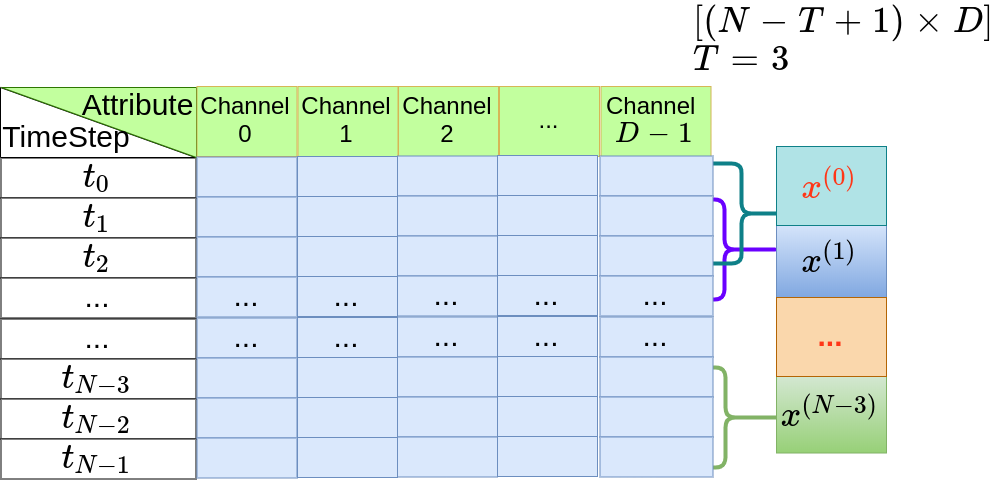
\includegraphics[width=1.0\textwidth]{labeling.png}
    \centering
	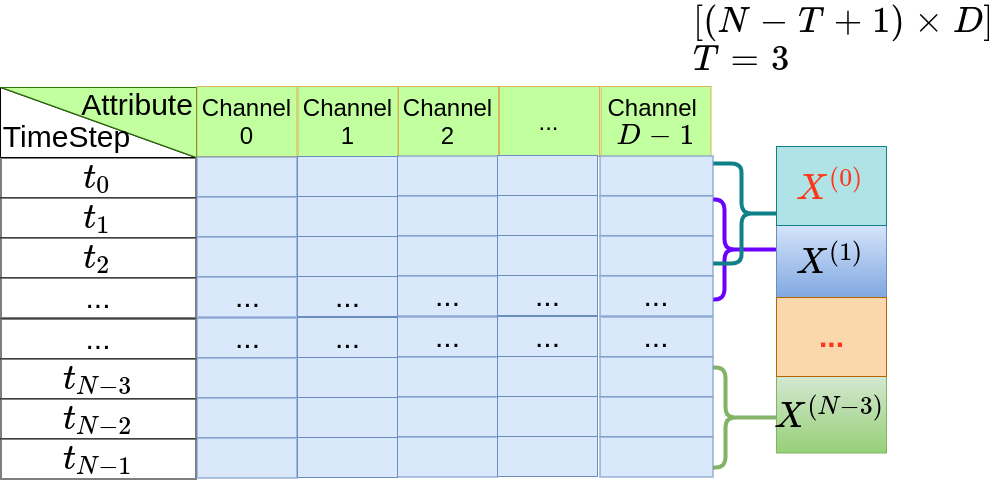
\includegraphics[width=.8\textwidth]{figures/labeling.png}
	\caption{Đánh nhãn dữ liệu}
	\label{fig:Labeling}

\end{figure}


Với các tham số:
\begin{itemize}
    \item $D$: Số thuộc tính của mỗi phiên giao dịch
    \item $T$: Số phiên giao dịch liên tiếp (Sliding window)
\end{itemize}

% \csvautotabular[respect 
%\resizebox{\textwidth}{!}{%
%	\csvautotabular[respect all]{figures/short_len_data.csv}
%}\\\\


% \makeatletter
% \csvset{
% 	autotabularcenter/.style={
% 		file=#1,
% 		after head=\csv@pretable\begin{tabular}{|*{\csv@columncount}{c|}}\csv@tablehead,
% 			table head=\hline\csvlinetotablerow\\\hline,
% 			late after line=\\,
% 			table foot=\\\hline,
% 			late after last line=\csv@tablefoot\end{tabular}\csv@posttable,
% 		command=\csvlinetotablerow},
% 	autobooktabularcenter/.style={
% 		file=#1,
% 		after head=\csv@pretable\begin{tabular}{*{\csv@columncount}{c}}\csv@tablehead,
% 			table head=\toprule\csvlinetotablerow\\\midrule,
% 			late after line=\\,
% 			table foot=\\\bottomrule,
% 			late after last line=\csv@tablefoot\end{tabular}\csv@posttable,
% 		command=\csvlinetotablerow},
% }
% \makeatother
% \newcommand{\csvautotabularcenter}[2][]{\csvloop{autotabularcenter={#2},#1}}
% \newcommand{\csvautobooktabularcenter}[2][]{\csvloop{autobooktabularcenter={#2},#1}}

% \csvautotabular[respect all]{figures/short_len_data_1.csv}\\\\

% \csvautotabular[respect all]{figures/short_len_data_2.csv}\\\\
% \section{Mô tả dữ liệu}

% Với phiên giao dịch dòng 1 SRN/BTC được ghi lại thành một dòng với thông tin như sau:\\
 
% \begin{itemize}
% 	\item symbol: Tên giao dịch giữa hai đồng với nhau cụ thể là đồng SRN so với đồng BTC
% 	\item Market: Tên sàn giao dịch cụ thể là sàn huopipro
% 	\item timeIndicator: Thời điểm mở phiên giao dịch 8 giờ 13/12/2018 UTC
% 	\item openPrice: Tỷ giá thời điểm mở phiên
% 	\item openPrice: Tỷ giá thời điểm đóng phiên
% 	\item highPrice: Tỷ giá cao nhất phiên giao dịch
% 	\item lowPrice: Tỷ giá thấp nhất phiên giao dịch
% 	\item volume: Khối lượng giao dịch (Ví dụ symbol là SRN/BTC volume có nghĩa là số đồng SRN)
% 	\item minTimestamp, maxTimestamp: do mỗi giao dịch cần một thời gian nhất định nên cần có thời gian bắt đầu và kết thúc giao dịch tính theo POSIX time.
% \end{itemize}
